\documentclass[fontset=macnew]{ctexart}
\usepackage{fontawesome}
\usepackage{fontspec}
\usepackage{bbding}
\usepackage{amsmath}
\usepackage{amsfonts}
\usepackage{ulem}
\usepackage{wasysym}
\usepackage{makeidx}
\usepackage{graphicx}
\usepackage{setspace}
\usepackage{tabu}
\usepackage{paralist}
\usepackage{lastpage}
\usepackage{enumerate} 
\usepackage{enumitem}
\usepackage{newtxtext}
\usepackage{mathptmx}
\usepackage{xpatch}
\usepackage{CJKfntef}
\usepackage{mhchem}
\usepackage{extarrows}
\usepackage{linalg}
\usepackage{makecell}
\usepackage{graphicx}
% 数学支持
\usepackage{amsmath, amssymb}
\usepackage{upgreek}

% 制定更多颜色

\usepackage{color}
\definecolor{yellowgreen}{RGB}{253, 204, 138}
\definecolor{qinglan}{RGB}{0, 255, 255} 
\definecolor{qinglv}{RGB}{20, 176, 228} 

% 设置页边距
\usepackage{geometry}

% 设置背景图片
\usepackage{graphicx}
\usepackage{eso-pic}

\newcommand{\tr}[1]{\hspace{-0.3em} \textcolor{red}{#1}\hspace{0.1em}} 
\newcommand{\tq}[1]{\textcolor{teal}{#1}}
\newcommand{\tb}[1]{\textcolor{blue}{#1}}
\newcommand{\trq}[1]{\textcolor{red}{#1}}

\newcommand{\point}[1]{\kh{#1分}}
\newcommand{\kh}[1]{\hspace{-0.1cm}(\hspace{-0.1cm}#1\hspace{-0.1cm})\hspace{-0.1cm}}
\newcommand{\khi}[1]{\hspace{-0.1cm}(\hspace{-0.1cm}#1\hspace{-0.1cm})\hspace{-0.3cm}}
\newcommand{\dkh}[1]{\hspace{-0.1cm}【\hspace{-0.1cm}#1\hspace{-0.1cm}】\hspace{-0.1cm}}
\makeatletter
\SetLabelAlign{hang}{%
	#1%
	\aftergroup\adjustparshapeindent}
%% 编号 #1 会通过 \sbox 存到 \@tempboxa 中,为避免全局设置,
%% 需要用 \aftergroup 跳到盒子外部来设置
\newcommand*\adjustparshapeindent{%
	\@ifnextchar\egroup
	{\aftergroup\adjustparshapeindent}
	{\adjustparshapeindent@auxi}}
\newcommand*\adjustparshapeindent@auxi{%
	\unless\ifdim\wd\@tempboxa=\labelwidth
	\adjustparshapeindent@auxii
	\fi}
%% 调整 \parshape 的缩进
\newcommand*\adjustparshapeindent@auxii{%
	\dimen@ = \dimexpr\wd\@tempboxa-\labelwidth\relax
	\labelwidth = \wd\@tempboxa
	\advance\linewidth -\dimen@
	\advance\leftmargin \dimen@
	\advance\@totalleftmargin \dimen@
	\parshape \@ne \@totalleftmargin \linewidth}

\setlist[enumerate]{
	%leftmargin=2em,%列表整体左缩进
	itemindent=0em,%条目首行缩进
	start=1,%开始序号
	parsep=0.2em,
	topsep=0.1em,%列表与上下文本间距
	itemsep=0.1em,%条目间距
	align=right}

\makeatother

\newcommand{\yssm}{第~\thepage~页\kh{共~\pageref{LastPage}~页}}
\usepackage{fancyhdr}
\renewcommand{\headrulewidth}{0pt}
\pagestyle{fancy}
\setlength{\footskip}{0.1cm}
\newlength{\lxsd}
\newcommand{\xg}[2]{
	\settowidth{\lxsd}{#1\ }
	\hangafter 1
	\hangindent \lxsd
	\noindent #1\ #2
}
\newcommand{\tih}[2]{
	\settowidth{\lxsd}{\textbf{#1}}
	\hangafter 1
	\hangindent \lxsd
	\noindent \textbf{#1}\,\textbf{#2}
}
\newcommand{\tikh}[2]{
	\settowidth{\lxsd}{\textbf{\kh{#1}}\,}
	\hangafter 1
	\hangindent \lxsd
	\noindent \textbf{\kh{#1}}\,\textbf{#2}
}
\usepackage{ifthen}

\newlength{\la}
\newlength{\lb}
\newlength{\lc}
\newlength{\ld}
\newlength{\laa}
\newlength{\lbb}
\newlength{\lcc}
\newlength{\ldd}
\newlength{\lee}
\newlength{\lf}
\newlength{\lhalf}
\newlength{\lquarter}
\newlength{\lmax}
\newcommand{\xx}[4]{\\[.5pt]%  
	\settowidth{\la}{A.~\,#1~~~}  
	\settowidth{\lb}{B.~\,#2~~~}
	\settowidth{\lc}{C.~\,#3~~~}  
	\settowidth{\ld}{D.~\,#4~~~}
	\settowidth{\laa}{A. }  
	\settowidth{\lbb}{B. }
	\settowidth{\lcc}{C. }  
	\settowidth{\ldd}{D. }
	\ifthenelse{\lengthtest{\la > \lb}}
	{\setlength{\lmax}{\la}}{\setlength{\lmax}{\lb}}  
	\ifthenelse{\lengthtest{\lmax < \lc}}  {\setlength{\lmax}{\lc}}  {}  \ifthenelse{\lengthtest{\lmax < \ld}}  {\setlength{\lmax}{\ld}}  {} 
	\setlength{\lhalf}{0.5\linewidth} 
	\setlength{\lquarter}{0.25\linewidth}
	\ifthenelse{\lengthtest{\lmax > \lhalf}}  
	{\vspace{-0.6cm}
		\begin{enumerate}[align=hang]
			\item[A.]#1
			\item[B.]#2
			\item[C.]#3
			\item[D.]#4
		\end{enumerate}
	}  {\ifthenelse{\lengthtest{\lmax > \lquarter}}  
		{\noindent
			\makebox[\lhalf][l]{A.~\,#1~~~}% 
			\makebox[\lhalf][l]{B.~\,#2~~~}\\%
			\makebox[\lhalf][l]{C.~\,#3~~~}%
			\makebox[\lhalf][l]{D.~\,#4~~~}}% 
		{\noindent\makebox[\lquarter][l]{A.~\,#1~~~}%
			\makebox[\lquarter][l]{B.~\, #2~~~}%
			\makebox[\lquarter][l]{C.~\, #3~~~}%      
			\makebox[\lquarter][l]{D.~\, #4~~~}}
}}

\newcommand{\xxiii}[3]{\\[.5pt]%  
	\settowidth{\la}{A. #1~~~}  
	\settowidth{\lb}{B. #2~~~}
	\settowidth{\lc}{C. #3~~~}  
	\ifthenelse{\lengthtest{\la > \lb}}
	{\setlength{\lmax}{\la}}{\setlength{\lmax}{\lb}}  
	\ifthenelse{\lengthtest{\lmax < \lc}}{\setlength{\lmax}{\lc}}{}  
	\setlength{\lhalf}{0.5\linewidth}
	\setlength{\lquarter}{0.25\linewidth}
	\ifthenelse{\lengthtest{\lmax > \lhalf}}
	{\noindent{}A. #1 \\ B. #2 \\ C. #3 }{  \ifthenelse{\lengthtest{\lmax > \lquarter}}  
		{\noindent
			\makebox[\lhalf][l]{A. #1~~~}% 
			\makebox[\lhalf][l]{B. #2~~~}\\%
			\makebox[\lhalf][l]{C. #3~~~}}% 
		{\noindent
			\makebox[\lquarter][l]{A. #1~~~}% 
			\makebox[\lquarter][l]{B. #2~~~}%     
			\makebox[\lquarter][l]{C. #3~~~}}
}}

\newcommand{\xxv}[5]{\\[.5pt]%  
	\settowidth{\la}{A. #1~~~}  
	\settowidth{\lb}{B. #2~~~}
	\settowidth{\lc}{C. #3~~~} 
	\settowidth{\ld}{D. #4~~~}  
	\settowidth{\lee}{E、#5~~~}   
	\ifthenelse{\lengthtest{\la > \lb}}
	{\setlength{\lmax}{\la}}{\setlength{\lmax}{\lb}}  
	\ifthenelse{\lengthtest{\lmax < \lc}}  {\setlength{\lmax}{\lc}}  {} 
	\ifthenelse{\lengthtest{\lmax < \ld}}  {\setlength{\lmax}{\ld}}  {} 
	\ifthenelse{\lengthtest{\lmax < \lee}}  {\setlength{\lmax}{\lee}}  {} 
	\setlength{\lhalf}{0.5\linewidth} 
	\setlength{\lquarter}{0.25\linewidth}
	\ifthenelse{\lengthtest{\lmax > \lhalf}}  
	{\noindent{}A. #1 \\ B. #2 \\ C. #3 \\ D. #4 \\ E、#5}  {  \ifthenelse{\lengthtest{\lmax > \lquarter}}  
		{\noindent
			\makebox[\lhalf][l]{A. #1~~~}% 
			\makebox[\lhalf][l]{B. #2~~~}\\%
			\makebox[\lhalf][l]{C. #3~~~}%
			\makebox[\lhalf][l]{D. #4~~~}\\%
			\makebox[\lhalf][l]{E、#5~~~}}% 
		{\noindent
			\makebox[\lquarter][l]{A. #1~~~}% 
			\makebox[\lquarter][l]{B. #2~~~}%     
			\makebox[\lquarter][l]{C. #3~~~}%
			\makebox[\lquarter][l]{D. #4~~~}\\%
			\makebox[\lquarter][l]{E、#5~~~}}
}}

\newcommand{\xxvi}[6]{\\[.5pt]%  
	\settowidth{\la}{A. #1~~~}  
	\settowidth{\lb}{B. #2~~~}
	\settowidth{\lc}{C. #3~~~} 
	\settowidth{\ld}{D. #4~~~}  
	\settowidth{\lee}{E、#5~~~}
	\settowidth{\lf}{E、#6~~~}     
	\ifthenelse{\lengthtest{\la > \lb}}
	{\setlength{\lmax}{\la}}{\setlength{\lmax}{\lb}}  
	\ifthenelse{\lengthtest{\lmax < \lc}}  {\setlength{\lmax}{\lc}}  {} 
	\ifthenelse{\lengthtest{\lmax < \ld}}  {\setlength{\lmax}{\ld}}  {} 
	\ifthenelse{\lengthtest{\lmax < \lee}}  {\setlength{\lmax}{\lee}}  {}
	\ifthenelse{\lengthtest{\lmax < \lf}}  {\setlength{\lmax}{\lf}}  {}  
	\setlength{\lhalf}{0.5\linewidth} 
	\setlength{\lquarter}{0.25\linewidth}
	\ifthenelse{\lengthtest{\lmax > \lhalf}}  
	{\noindent{}A. #1 \\ B. #2 \\ C. #3 \\ D. #4 \\ E、#5 \\ F、#6}  {  \ifthenelse{\lengthtest{\lmax > \lquarter}}  
		{\noindent
			\makebox[\lhalf][l]{A. #1~~~}% 
			\makebox[\lhalf][l]{B. #2~~~}\\%
			\makebox[\lhalf][l]{C. #3~~~}%
			\makebox[\lhalf][l]{D. #4~~~}\\%
			\makebox[\lhalf][l]{E、#5~~~}%
			\makebox[\lhalf][l]{F、#6~~~}}% 
		{\noindent
			\makebox[\lquarter][l]{A. #1~~~}% 
			\makebox[\lquarter][l]{B. #2~~~}%     
			\makebox[\lquarter][l]{C. #3~~~}%
			\makebox[\lquarter][l]{D. #4~~~}\\%
			\makebox[\lquarter][l]{E、#5~~~}%
			\makebox[\lquarter][l]{F、#6~~~}}%
}}

%填空题画线  \tk
%\newcommand{\tk}[2][2.5]{\; \underline{\hspace{#1 cm} \hphantom{#2} \hspace{#1 cm} } \, }
\newcommand{\note}{\textcolor{blue}{\faBook} \phantom{h}}

%判断题后面加括号
\newcommand{\pd}[2][1]{\nolinebreak\dotfill\mbox{\raisebox{-1.8pt}
		{$\cdots$}(\makebox[#1 cm][c]{
			\ifthenelse{\boolean{print}}
			{\ifthenelse{\equal{#2}{t}}{\Checkmark}{\XSolid}}
			{}
		})}}

\newboolean{print}
\setboolean{print}{true}

\usepackage{ulem}
\newcommand{\tk}[2][0.5]{\;\uline{ 
		\hspace*{#1 cm}
		\ifthenelse{\boolean{print}}{#2}{\hphantom{#2}}  
		\hspace*{#1 cm}
} }

\newcommand{\jd}[2][4]{\par
	\begin{minipage}[t][#1cm][t]{0.92\linewidth}	
		\ifthenelse{\boolean{print}}{#2}{}  
	\end{minipage} 
}	

\usepackage{pifont}
\setboolean{print}{false}


% 中文字体是 思源黑体
%\setCJKmainfont{SourceHanSansCN-Normal}

% 设置英文字体
\setmainfont{texgyrepagella-regular.otf} 


\newcommand\BackgroundPic{
\put(0,0){
\parbox[b][\paperheight]{\paperwidth}{%
\vfill
\centering
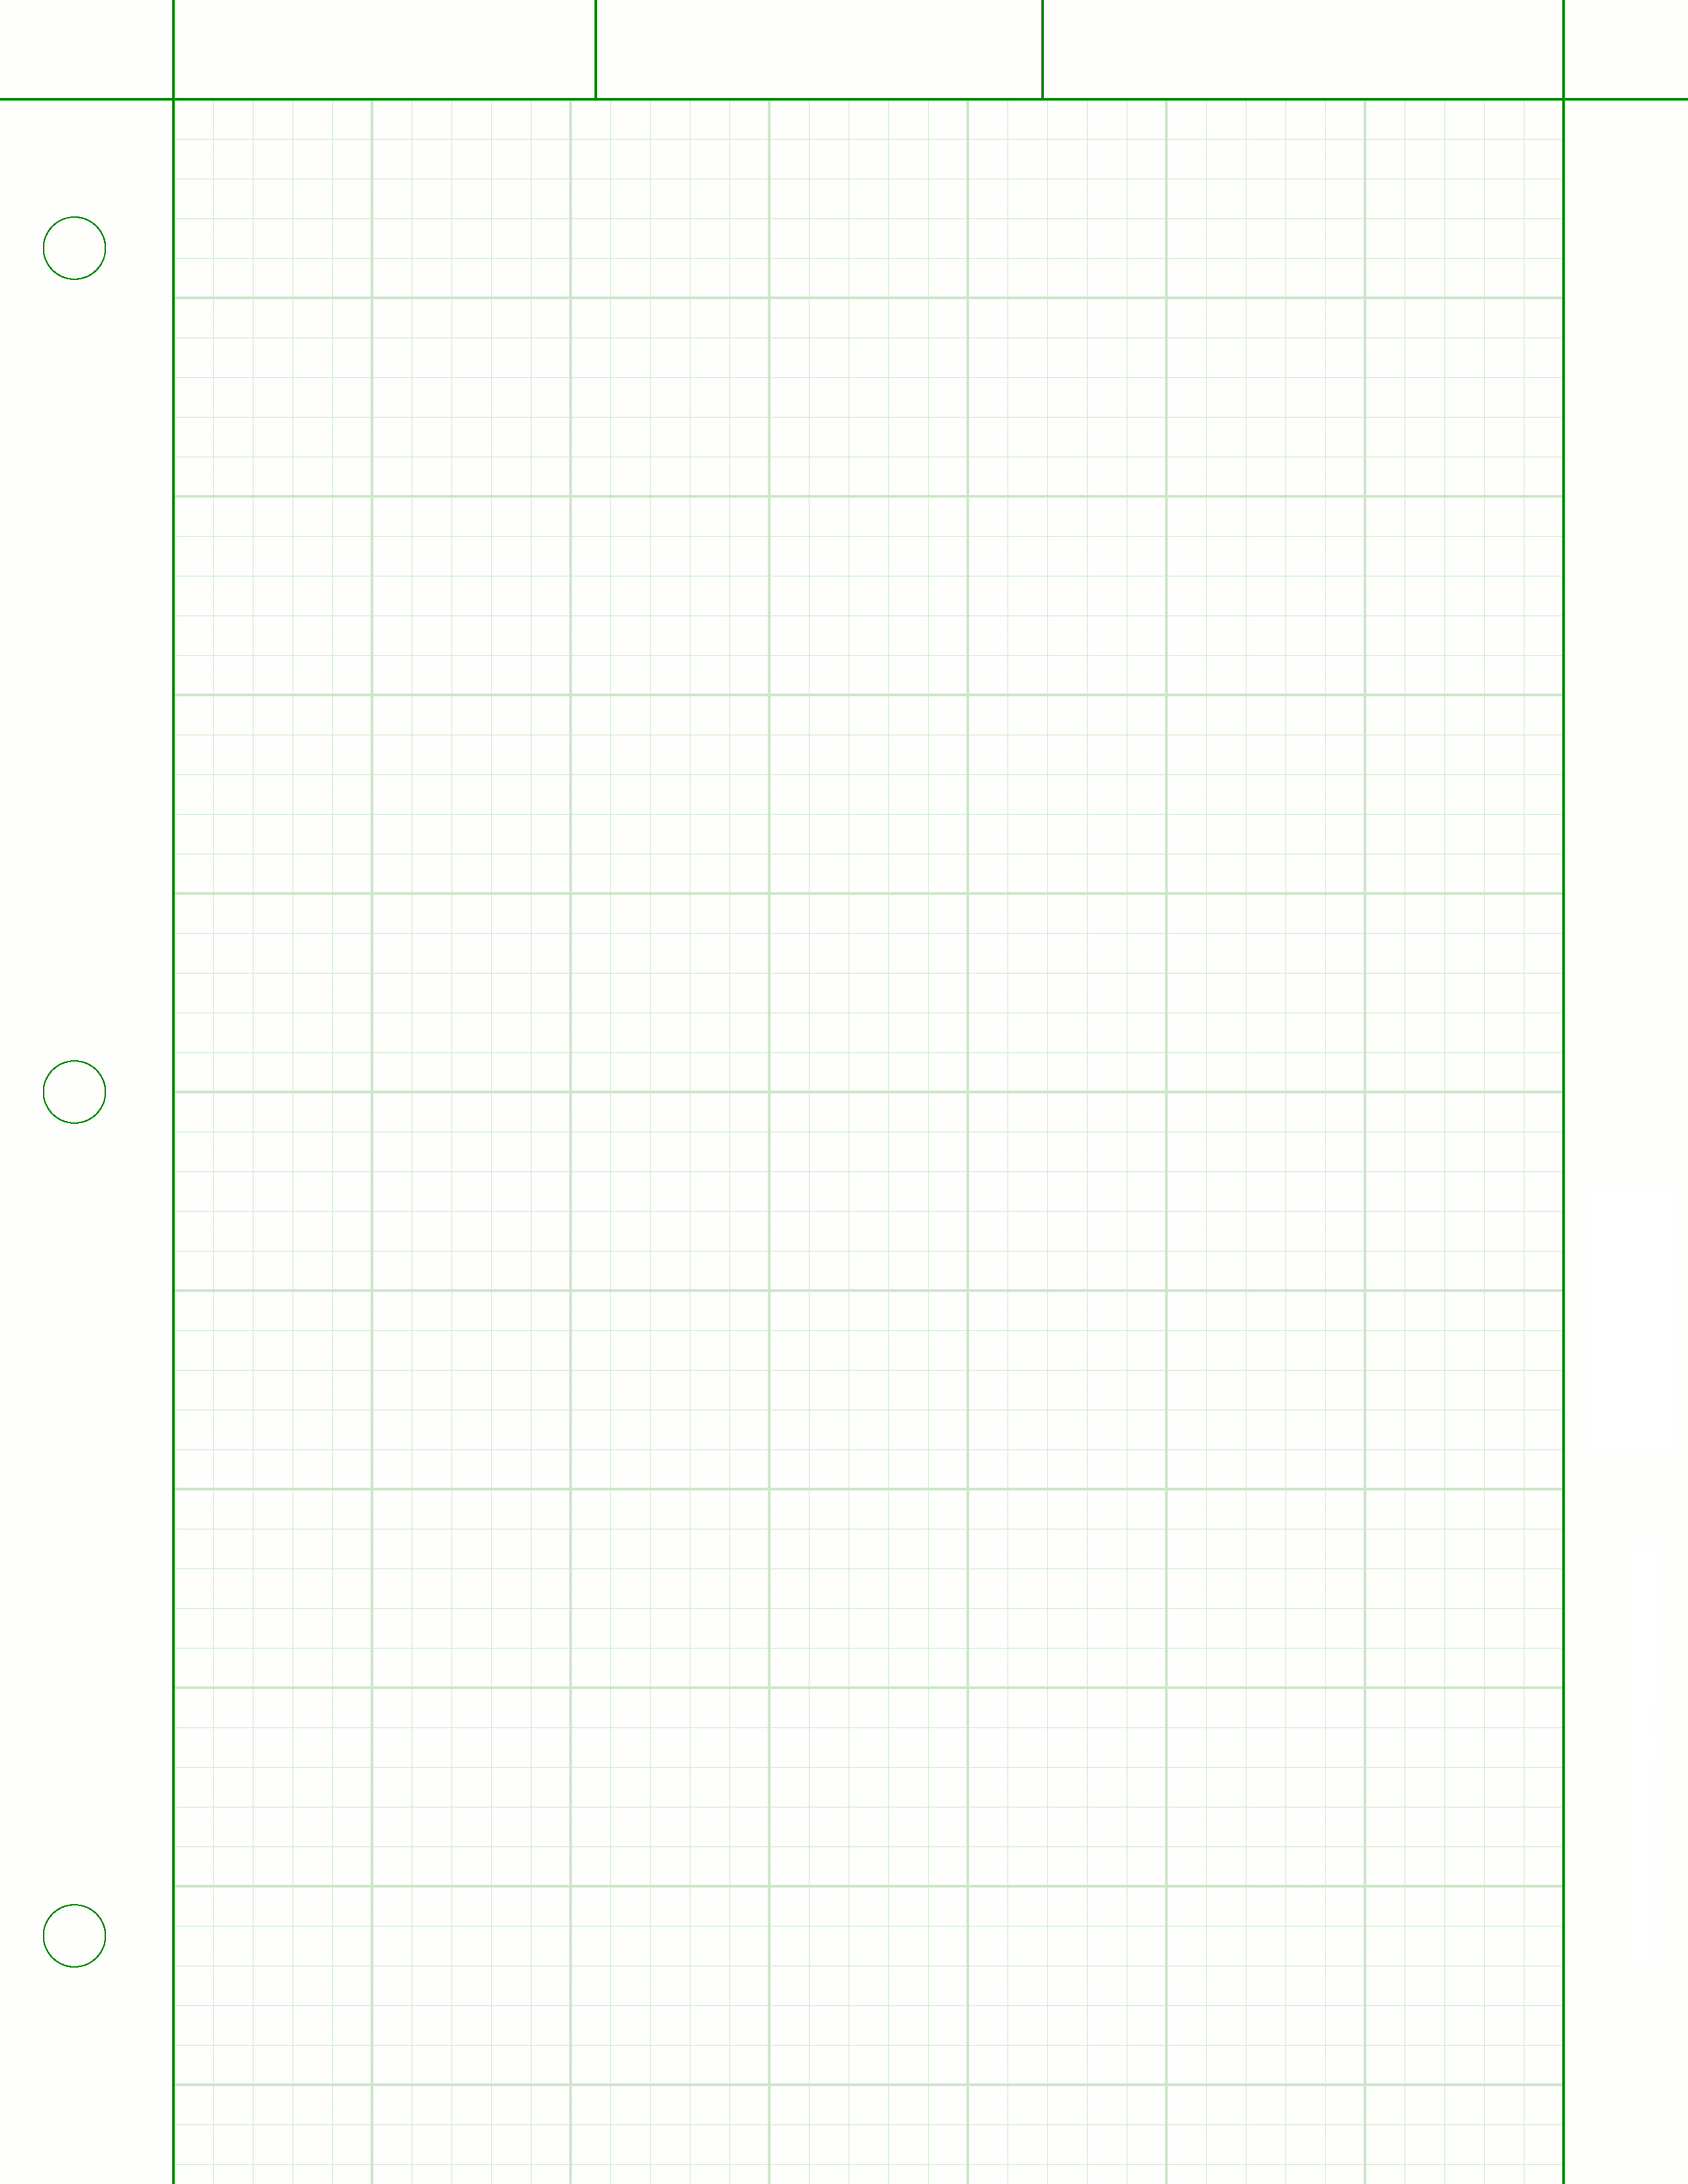
\includegraphics[width=\paperwidth,height=\paperheight,
keepaspectratio]{background.png}%
\vfill
}}}


\begin{document}
\newgeometry{left=3cm, right=3cm,bottom=2.5cm,top=2.5cm}
\AddToShipoutPicture{\BackgroundPic}
\begin{center}
	\fontsize{20pt}{12pt}\selectfont 政治二刷选择题错题每天整理
\end{center}


%马哲部分
% !TEX encoding = UTF-8
\section{马哲部分}

\textcolor{red}{\faBook 马哲的部分最多也最难,需要理解的东西最多,也需要充分的理解才能做好题目。}

\begin{enumerate}[align=hang, start=1]
	%第一题
	\item 为马克思主义的产生提供了自然科学前提的有 
	\xx{相对论}{\textcolor{red}{细胞学说}}{\textcolor{red}{能量守恒与转化定律}}{\textcolor{red}{生物进化论}}%选择题调用直接使用本方式,会有自动缩进,也会有自动判断长度选择相应的形式
	\note 直接记住结论接可以了。
	
	
	%第二题
	\item 下列命题中,属于客观唯心主义哲学观点的有 
	\xx{物是感觉的复合}{世界是观念的集合}{\textcolor{red}{世界是绝对观念的外化}}{\textcolor{red}{世界是上帝意志的创造物}}%选择题调用直接使用本方式,会有自动缩进,也会有自动判断长度选择相应的形式
	\note B选项中的感觉是人的感觉,客观唯心把虚构出来的在人存在的客观精神当作世界的本原。
	
	
	%第三题
	\item 形而上学唯物主义物质观的缺陷在于
	\xx{\textcolor{red}{把某种特殊的物质形态误认为物质的一般}}{\textcolor{red}{割裂了自然界与人类社会的物质统一性}}{否认意识由物质决定}{\textcolor{red}{不了解人类对物质的认识是一个永无止境的发展过程}}%选择题调用直接使用本方式,会有自动缩进,也会有自动判断长度选择相应的形式
	\note 形而上学唯物主义把物质归结为原子,混淆了物质结构概念同哲学的物质范畴的区别,\textcolor{teal}{不了解人类对物质的认识是一个永无止境的发展过程。}把某种特殊的物质形态误认为物质的一般。\textcolor{teal}{割裂了自然界与人类社会的物质统一性}。
	
	
	%第四题
	\item 马克思主意的物质观认为,客观实在性是物质的唯一特性,既肯定了哲学物质范畴同自然科学物质结构理论的联系,又把它们区别开来,体现了唯物论和辩证法的统一,克服了形而上学唯物主义的缺陷。马克思主义物质观所体现的唯物辩证法是指
	\xx{\textcolor{red}{从个性中看到共性}}{\textcolor{red}{从相对中找到绝对}}{\textcolor{red}{从暂时中发现永恒}}{从局部中看到整体}
	\note 考研政治中,共性和个性、矛盾的普遍性和特殊性、一般和个别可以视为同一个层次的概念,而整体与部分是另一个层次的概念。
	
	
	%第五题
	\item 
	恩格斯于1820年11月28日出生在德国巴西门市的一个工厂主家庭。他称自己一生所做的事就是`` 拉第二小提琴''。恩格斯不仅与马克斯一起创立马克思主义,参加并指导国际工人运动,而且在传播和发展马克思主义方面做出了杰出的贡献。恩格斯全面阐述马克思主义理论体系的著作是 
	\xx{ 《共产党宣言》  }  {  《家庭、私有制和国家的起源》  }  {  \textcolor{red}{《反杜林论》}   }  { 《自然辩证法》   }
	\note  《德法年鉴》论文的发表->唯心主义向唯物主义、革命民主主义向共产主义转变,奠定了\textcolor{red}{思想前提} ,《德意志形态》->第一次比较系统的阐述了历史唯物主义的基本原理。《共产党宣言》->\textcolor{red}{马克思主义的公开问世}。 《资本论》-> 最厚重、最丰富的著作,被誉为\textcolor{red}{``工人阶级的圣经''}。《反杜林论》->全面阐述马克思主义理论体系,被称为\textcolor{red}{马克思主义的``百科全书''。}
	
	
	%第六题
	\item 
	2019年4月10日21时,全球多国科研人员合作的``世界视界望远镜''项目在全球六地同步举行发布会,发布了世界上首张黑洞图像,公布了人类首次拍到的黑洞照片。这是继2015年人类通过引力波探测``听到''两个黑洞合体之后,证明黑洞存在的直接``视界''证据。有科学家认为,这张看起来有点模糊的照片意义非凡,它再次验证了爱因斯坦广义相对论的语言是对的,并将进一步帮助科学家解答演化等一系列宇宙本质问题。人类首次``看到黑洞正面照表面'' 
	\xx{\textcolor{red}{空间的性质依赖于物质的分布及运动状态} }{\textcolor{red}{世界是物质的统一体}}{物质世界的客观存在与人的实践和认识水平有关}{\textcolor{red}{空间的观念随人的认识发展而拓展}}
	\note 没选D,\textcolor{teal}{物质运动和空间的客观实在是绝对的,物质运动时间和空间的具体特性是相对的。}
	%第七题
	\item 鲁迅说过:``描神画鬼,毫无对证,本可以专靠神思,所谓`天马行空'地挥写了。然而他们写出的却是三只眼、长颈子,也就是在正常的人体上增加了眼睛一只,拉长了颈子两三尺而已。''这段话说明,人们头脑中的鬼神观念
	\xx{ 是头脑中主观自生的  }{	\textcolor{red}{  是人脑对客观世界的歪曲反映 }   }{是人脑对鬼神的虚幻反映}{	\textcolor{red}{  可以从人世间找到它的原型 }} 
	\note  \textcolor{teal}{意识的主观性不仅表现为它对客观事物近似真实的反映,而且还可能表现为它是对客观对象的歪曲的或是虚幻的反映,但这种歪曲的或是虚幻的反映,也是对客观对象的反映,有其客观的``原型''}。歪曲反映而非虚幻反映,同时这种形象是人按照自己形象塑造出来的,而非头脑产生的,鬼神不是客观对象,所以不肯呢个是虚幻反映。
	\textcolor{blue}{意识,不管正确错误、先进落后,都是物质世界的主观映像。人的意识不管主观色彩多么浓厚,归根到底都有自己的客观``原型''}。
	
	
	\item 
	马克思说:``蜘蛛的活动和织工的活动相似,蜜蜂建筑蜂房的本领使人间的许多建筑师感到惭愧。但是最蹩脚的建筑师比最灵巧的秘方高明的地方,是他在用蜂蜡筑蜂房前,已经在自己的头脑中把它建成了。''这句话说明
	\xx   {\textcolor{red}{主观能动性是人区别于动物的特征}}{	\textcolor{red}{ 人的时间活动是有意识、有目的的 } }  
	{\textcolor{red}{人以自己的活动来改造世界,而动物只能以本能来适应环境 } }  {意识先于物质、决定物质}	
	\note 没选C项,\tq{与动物本能的、被动的适应性活动不同,人类的实践活动是一种有意识、有目的的活动,人以自己的活动来改造世界,而动物只能以本能来适应环境,主观能动性是人区别于动物的特征}。\tb{高级动物也有感觉和心理,但只有人才有意识。实践、意识都是人特有的,动物、机器人都没有}。\tb{同时人脑是意识的器官,但不是源泉,意识的源泉是客观世界}。
	
	
	%第9题
	\item 
	从物质与精神的关系来看,``画饼不能充饥''这是因为
	\xx{精神与物质不具有同一性}{精神对物质具有相对独立性}{\tr{观念的东西不能代替物质的东西}}{\tr{事物是人脑的反映不等同于事物自身}} 
	\note B项本身说法正确,但不符合题意,\tb{考研政治范围内,相对独立性是指,A决定B,但是B又具有自己特有的发展形式和规律,例如B的变化发展与A的变化发展不同步,B对A具有反作用等。}
	
	
	%第10题
	\item 
	马克思在《德意志意识形态》中写到:``因此,在这样的场合费尔巴哈从不谈人的世界,而是每次都求救于外部自然界,而且是那个尚未置于人的统治之下的自然界。但是,每当有了一项新的发明,每当工业向前前进一步,就有一块心的地盘从这个领域划出去,而能用来说明费尔巴哈这类论点的事例借以产生的基地,也越来越小了。''对这段话理解正确的有
	\xx{  \trq{自在自然日益转化为人化自然}}{\trq{实践是使物质世界分化为自然界与人类社会的历史前提和二者统一起来的现实基础}}{自然界不再具有客观实在性}{\trq{人类社会的存在和发展影响并不断改变着自然}} 
	\note 漏选了A,\tq{在实践活动过程中,物质世界被区分为自然界和人类社会两大领域。自然界是人生活于其中的客观世界,其中一部分是人类活动尚未触及的\tb{自在自然},另一部分是打上人类活动印记的\tb{人化自然}}。``每当工业前进一步,就有一块新的地盘转化为人化自然。A正确''。\tb{实践是物质世界分化为自然界与人类社会的\trq{历史前提},又是自然界与人类社会统一起来的\trq{现实基础}}。
	
	%第11题
	\item 
	陕西榆林地处于毛乌素沙漠边缘,当地凭借技术创新,把大片的荒沙地改成了高效农田。土地由坏变好,源于陕西省在沙漠治理上的技术创新。研究人员发现,毛乌素沙漠中含有大量的沙岩和沙子,这两种物质只要比例调配得当,就能改造好荒沙地/沙荒地改造的成功说明
	\xx{合理改造自然规律是人与自然和谐相处的关键}{科技创新是社会发展的根本动力}{\trq{认识世界是为了改造世界}}{\trq{人类可以通过劳动实践协调人与自然的关系}}
	\note \tq{规律是客观的,人既不能创造也不能改造自然},A中 \trq{改造} 两个字错了,\trq{社会基本矛盾}是社会发展的根本动力,\trq{阶级斗争、社会革命、改革、科技创新}是阶级社会发展的\trq{重要动力}。
	
\end{enumerate}


%毛概部分
% !TEX encoding = UTF-8
%毛概
\section{毛概部分}
\textcolor{red}{\faBook 毛概的部分很多也很难,需要记忆的东西最多,习是真的能写。}
\begin{enumerate}[align=hang, start=1]
	%第一题
	\item 1938年,毛泽东在党的六届六中全会上作的题为《论新阶段》的政治报告中,最先提出了``马克思主义中国化''的命题。毛泽东提出要实现马克思主义的中国化,源于
	\xx{对马克思主义的深刻理解}{对中国国情的准确把握}{\textcolor{red}{对中国革命进程中正反两个反面的实践经验的科学总结}}{对当时时代主题的清晰判断}
	\note B、C选项容易纠结不清楚,三短一长选最长吧。
	
	%第二题
	\item 下列各项中,体现毛泽东思想在解放战争时期和新中国成立以后继续得到发展的有
	\xx{\textcolor{red}{提出了人民民主专政的理论}}{\textcolor{red}{提出了社会主义改造和建设社会主义制度的基本方略 }}{\textcolor{red}{ 提出了要把马克思主义的基本理论同中国革命和建设具体相结合的``第二次结合''}}{\textcolor{red}{ 提出了关于正确处理人民内部矛盾的理论}}
	\note 漏选了C项,精练精讲有明确的回答,P105。
	
	%第三题
	\item 毛泽东提出,中国共产党区别于其他任何政党的显著标志是 
	\xx {  \textcolor{red}{理论和实践相结合的作风}  } { 
		\textcolor{red}{和人民群众紧密联系在一起的作风} }    { \textcolor{red}{自我批评的作风} }   { 谦虚、谨慎、不骄、不躁的作风 }
	\note 而区别于任何政党的标志是毛泽东在党的七大作的 \trq{《论联合政府》}中指出的。区别于任何政党的标志是A、B、C三项,而D是``两个务必''的内容,\textcolor{teal}{即``务必使同志们继续保持谦虚、谨慎、不骄、不躁''的作风},\textcolor{teal}{务必使同志们继续地保持艰苦奋斗的作风},P121。
	
	%第四题
	\item 实事求是,就是一切从实际出发,理论联系实际,不断深化对中国国情的认识,找出适合中国情况的革命和建设道路,确定我们党领导人民改造中国、建设中国的战略策略,实现推动历史前进的目标。实事求是,是
	\xx {   	\textcolor{red}{ 马克思主义中国化理论成果的精髓和灵魂 }}    { 	\textcolor{red}{ 中国共产党人认识世界、改造世界的根本要求}  }    {	\textcolor{red}{ 中国共产党的基本思想方法、工作方法、领导方法 }   }  { 	\textcolor{red}{    马克思主义的根本观点}    }
	\note  漏选了D,记住它的面容。  
	
	%第五题
	\item 近代以来中华民族面临的两大历史任务是 
	\xx{ 推翻军阀官僚的反动统治  } { 	\textcolor{red}{ 争取民族独立和人民解放 }}  {建立无产阶级专政的政权}  { 	\textcolor{red}{ 实现国家富强和人民富裕 }}
	\note 错选了A,近代以来这个范围还是很广的。
	
	%第六题
	\item 中国革命的中心问题是
	\xx { 农民土地问题}{统一战线问题}{ 武装斗争问题}{\tr{领导权问题}}
	\note 民主革命的几个提法,  中国革命的\tr{中心问题}、新民主主义革命理论的\tr{核心问题}是\tr{无产阶级领导权},
	中国革命的\tr{基本问题}是\tr{农民问题},新民主主义革命的\tr{主要内容},\tb{没收封建地主阶级的土地归农民所有},
	新民主主义革命的\tr{实质}是,\tb{中国共产党领导下的农民革命},新民主主义革命的\tr{首要问题是}\tb{分清敌友}。
	
	\item 
	工人阶级实现革命领导权的基础是
	\xx{\tr{对农民阶级的领导}}{对于小资产阶级的领导}{对于民族资产阶级的领导}{对于军队的领导} 
	\note 记住她
	
	%第八题
	\item  ``因为中国资产阶级根本上与剥削农民的豪绅地主相联合相混合,中国革命要推翻豪绅地主阶级,便不能不同时推翻资产阶级。''这一观点属于
	\xx{ \tr{``毕其功于一役''的观点}}{``二次革命''的观点}{民主主义革命是社会主义革命必要准备的观点}{中国革命分``两步走''的观点}
	\note ``毕其功于一役'',\tb{混淆了新民主主义革命和社会主义革命的界限},是一种\tr{``左倾主义''}的观点,``两步走'',\tb{割裂了新民主主义革命和社会主义革命的联系},是一种\tr{``右倾主义''}的观点。
	
	%第9题
	\item 
	新民主主义革命理论的核心问题是
	\xx{分清敌友}{农民问题}{\tr{无产阶级领导权}}{土地问题}
	\note \tq{新民主主义革命理论的核心问题和中国革命的中心问题都是}\tr{无产阶级领导权的问题}。	
	
	%第10题
	\item 
	新民主主义革命理论形成的客观条件有
	\xx{\tr{旧民主主义革命的失败} }{ \tr{近代中国革命形式的发展} }{  对中国革命经验教训的概括和总结 }{ \tr{世界形式的新变化} }
	\note C项属于理论的东西不属于客观的条件。
	
	%第11题
	\item 
	无产阶级及其政党对中国革命的领导权不是自然而然得来的,而是在与资产阶级争夺领导权的斗争中实现的。毛泽东提出的无产阶级要实现对同盟者的领导必备的条件有。
	\xx{ \tr{率领同盟者向共同的敌人做坚决的斗争,并取得胜利}}{坚持发展进步势力,争取中间势力,孤立顽固势力的方针}{\tr{对同盟者以物质福利,至少不损害其利益,同时给予政治教育}}{对同盟者采取``有理、有利、有节''的策略原则}
	\note A、C项是毛泽东提出的``领导的阶级和政党,要实现自己对于被领导阶级、阶层、政党和人民团体的领导,具备的条件'',B是抗日战争中共巩固和扩大民族统一战线的总方针,D是抗日战争中对顽固派势力的总方针。
	
	%第12题
	\item 
	新民主主义经济纲领的内容是
	\xx{\tr{没收封建地主阶级的土地归农民所有}}{ \tr{没收官僚资产阶级的垄断资本归新民主主义的国家所有}}{\tr{保护民族工商业}}{没收外国在华资本归新民主主义的国家所有}
	\note 记住她就行
	
	%第13题
	\item 
	关于新民主主义政治纲领规定的新民主主义国家,以下说法正确的有
	\xx { \tr{国体是各革命阶级的联合专政}} {\tr{政体是民主集中制的人民代表大会制度}}{各革命阶级的联合专政是工农民主专政}{\tr{人民当家作主是新民主主义国家制度的核心内容和基本准则}}
	\note \tq{国体:}\tb{无产阶级领导的以工农联盟为基础,包括小资产阶级、民族资产阶级和其他反帝反封建的人们在内的各革命阶级的联合专政},\tq{政体:}\tb{民主集中制的人民代表大会制度}。
	
	%第14题
	\item 
	新民主主义文化就是无产阶级领导的人民大众的反帝反封建的文化,即民族的科学的大众的文化。其中``民族的'',就其内容说,是指 
	\xx{具有鲜明的民族风格、民族形式和民族特色}{具有中国作风和中国气派}{\trq{反对帝国主义压迫,主张中华民族的尊严和独立}}{ 反对封建思想和迷信思想}
	\note \tb{新民主主义文化是\trq{民族的},就其\trq{内容}说是反对帝国主义压迫,主张中华民族的尊严和独立,就其\trq{形式}是具有鲜明的民族风格、民族形式和民族特色,要有中国作风和中国气派。}\tq{新民主主义文化中居于指导地位的是共产主义思想,而非新民主主义思想。}
	
	%第15题
	\item 中国革命的特点和优点是
	\xx{由中国共产党领导的人民战争}{目标是争取民族独立、人民解放,最终实现国家的繁荣富强}{以反帝反封建作为两大革命任务}{\trq{以武装的革命反对武装的反革命}} 
	\note \tb{武装斗争是中国革命的特点和优点之一。}
	``三个'为一组的易混淆的考点 
	
	%表格总结
	\begin{center}
			\hspace{-1cm}
		\begin{tabular}{|c|c|c|}
			 \hline 
			 提出时间和著作      &        名称            &        内容    \\ 
			 \hline 
			 \makecell[c]{1981年十一届六中全会\\《历史决议》 }         &     毛泽东思想活的灵魂      & 独立自主、实事求是、群众路线 \\
			 \hline
			 																		&  \makecell[c]{中国革命走农村包围城市,\\ 武装夺取政权的道路的三个内容} &     \makecell[c]{土地革命、武装斗争\\农村革命根据地建设}		\\
			\hline 
			\makecell[c]{1939年\\《共产党人发刊词》}		& 新民主主义革命的三大法宝     &    \makecell[c]{统一战线、武装斗争\\ 党的建设}	\\			    
			\hline
			\makecell[c]{1935年七大  \\ {  《论联合政府》}}    &中国共产党的三大优良作风   &   \makecell[c]{理论联系实际、密切联系群众 \\批评与自我批评}			\\
			\hline
		\end{tabular}
	\end{center}
	
	
	%第16题
	\item 
	土地革命战争时期,毛泽东指出:``一国之内,在四周白色政权的包围中,有一块或若干小块红色政权的区域长期存在,这是世界各国从来没有的事。这种奇事的发生,有其独特的原因''。红色政权能够存在和发展的原因是
	\xx{ \trq{近代中国是多个帝国主义间接统治的半殖民地国家,社会政治经济发展极端不平衡}}{\trq{过敏革命的政治影响及良好的群众基础}}{\trq{全国革命形式的继续向前发展}}{\trq{相当力量正式红军的存在以及当的有力量及其正确的政策}}
	\note 必须区分好\trq{``必须走''}和\trq{``可以走''},必要性是由\trq{具体国情}决定的,\tb{内无民主制度,外无民族独立}
	以及\tb{中国是一个农业大国,农民占全国人口的绝大多数,是无产阶级可靠的同盟军和革命的\trq{主力军}}。
	而``可以走''是由\trq{特殊国情}决定的,即为题目选项,其中 ``半殖半封''提供了缝隙和可能、革命群众基础好、全国革命形式的继续发展提供了\trq{客观条件}、相当力量的红军则是\trq{坚实的后盾},党的正确政策则是重要的\trq{主观条件}。必须走的两条还分别回答了为什么必须 \trq{武装夺取政权}和\trq{农村包围城市}的问题。
	
	%第17题
	\item 
	中国革命必须建立最广泛的统一战线,这是由
	\xx{\trq{中国半殖民地和半封建社会的阶级状况决定的}}{半殖民地半封建地的中国社会的交织在一起的诸多矛盾决定的}{\trq{中国革命的长期性、残酷性及发展的不平衡性所决定的}}{战争与革命的时代主题决定的}
	\note  这是建立革命统一战线的\trq{必要性},而B选项则是可能性。
	
	%第18题
	\item 
	近代中国社会的阶级结构是``两头小中间大'',``中间是指'' 
	\xx{\trq{无产阶级}}{农民阶级}{\trq{民族资产阶级}}{城市小资产阶级}
	\note \tq``两头''一头是指 \trq{无产阶级},另一头指 \trq{地主大资产阶级},``中间''是指 \trq{农民、城市小资产阶级以及其他中间势力}。
	
	
	
\end{enumerate}

%近代史部分
% !TEX encoding = UTF-8
%近代史部分
\section{近代史}

\textcolor{red}{\faBook 近代史的部分相对比较简单,主要是土地、还有一些革命性质弄清楚,串联成线}


\begin{enumerate}[align=hang, start=1]
	
	%第一题
	\item 鸦片战争后中国\textcolor{red}{社会性质}发生的变化是	
	\xx{\textcolor{red}{ 独立的中国逐步成为半殖半封的中国 }} { 帝国主义和中华民族的矛盾成为主要矛盾 }  { \textcolor{red}{ 封建的中国逐步成为半封建地的中国 }  } {  反对帝国主义成为中国革命的主要任务 } 
	\note  主义是性质的变化,B、D两项都是矛盾的变化。
	
	%第二题
	\item 下列条约中涉及香港的有 
	\xx { \textcolor{red}{ 《南京条约》}}{ 《辛丑条约》 } { \textcolor{red}{ 《北京条约》}} {\textcolor{red}{《展拓香港界址条约》}}
 	\note 1842年南京条约,香港岛割让,1860年北京条约,割去香港岛对岸九龙半岛南端和昂船洲,1898年展拓香港界址条约被迫签署。
 	
	%第三题
 	\item 在近代,帝国主义列强不能共同瓜分中国和对中国实行直接殖民统治的原因在于
 	\xx{   	\textcolor{red}{   中国长期以来一直是一个统一的大国 } }{   	\textcolor{red}{   中国人民顽强、持久的反抗}    }  {     	\textcolor{red}{ 帝国主义列强之间争夺中国的矛盾无法协调  } }  {  中西文化存在着巨大差异  } 
 	\note 漏选A了,记住她的脸,不忘记。  
 	
 	%第四题
 	\item 
 	19世纪70年代以后,王韬、薛福成、马建忠、郑观应等人不仅主张学习西方的科学技术,同时也要求吸纳西方的政治、经济学说。他们共同的特点是具有
 	\xx{\tr{比较强烈的反对外国侵略的爱国思想}}{\tr{希望中国独立富强的爱国思想}}{追求实行民主共和的制度的思想}{\tr{一定程度反对封建专职的民主思想}}
	\note 没选D,记下来,\tq{一定程度反对封建专职的民主思想}也对。
	
	%第五题
	\item 
	19世纪90年代末中国出现戊戌维新运动不是偶然的,它的发生有着深刻的历史背景,主要是
	\xx{中国民族资本主义已经成为中国经济的主要形式}{\tr{新兴的民族资产阶级迫切要求中国发展资本主义开辟道路}}{\tr{甲午战争惨败造成的民族危机激发来新的民族觉醒}}{\tr{资产阶级改良思想在中国迅速传播}}
	\note \tb{即便到了后期,中国民资也没有成为中国经济的主要形式}。
	
	%第六题
	\item 
	洋务运动期间,洋务派兴办的民用企业中,采用官督商办的企业基本是
	\xx{买办官僚性质的}{封建主义的}{半封建地半殖民地的}{\trq{资本主义性质的}}
	\note 这些官督商办的民用企业,虽然受官僚的控制,发展受控制,但基本上\tq{资本主义性质的近代企业}
	
	%第七题
	\item 
	甲午战争一役,洋务派经营多年的北洋海军全军覆没,标志着以``自强''`求富`'为目标的洋务运动的失败。决定洋务运动必然失败命运的原因是
	\xx{洋务运动对外国具有依赖性}{洋务派通过所掌握的国家权力集中力量优先发展军事工业 }{\trq{洋务运动的指导思想是``中学为体,西学为用''}}{洋务运动的目标是``自强,求富''}
	\note \tq{洋务运动的指导思想是``中学为体,西学为用'',即在封建主义思想的指导下,在维持的上层建筑、经济基础的条件下发展一些近代企业,为维护清朝的封建统治服务。}
	
	%第八题
	\item 
	康有为等维新派自身的局限性主要表现在
	\xx{\trq{不敢否定封建主义}}{\trq{对帝国主义抱有幻想}}{不敢鼓吹民权}{\trq{惧怕人民群众}}
	\note 记住她就行了。
	
	%第九题
	\item 
	戊戌维新运动是一次爱过救亡运动,维新派在民族危亡的关键时刻
	\xx{\trq{高举救亡图存的旗帜}}{\trq{要求通过变法,发展资本主义,使中国走上富强的道路}}{成功地建立起存在百日的君主立宪制度}{\trq{其政治实践和思想理论,贯穿着强烈的爱国主义精神,推动了中华民族的觉醒}}
	\note 戊戌变法未能成功地建立起资本主义的君主立宪制。
	
	%第10题
	\item 
	包括孙中山在内的许多中国革命先驱者早年也尝试采取和平的手段来推进中国的变革与进步,但最终还是走上了决心以革命的方法推翻清王朝的道路。促使孙中山改变思想,认为和平改革不能解决中国的问题的原因是
	\xx{\trq{孙中山关于改革的上书没有得到重视}}{\trq{孙中山发现清朝的腐败比他原先了解的要严重的多}}{孙中山得到了共产国际和中国共产党的真诚帮助}{资产阶级革命派在与资产阶级改良派的论战中得到了胜利}
	\note C、D与题意无关。
		
\end{enumerate}

%思修部分
% !TEX encoding = UTF-8
%思修法基
\section{思修法基}
\textcolor{red}{\faBook 背就完事儿了}

\begin{enumerate}[align=hang, start=1]
	%第一题
	\item 法律是成文的道德,道德是内心的法律,法律和道德都具有规范社会行为、维护社会秩序的作用。以下既属于道德规范又是法律规范的是
	\xx{  	\textcolor{red}{  爱国主义 } }  {  	\textcolor{red}{  诚实守信 }   }   {  	\textcolor{red}{  尊重他人权利 }  }   {  	\textcolor{red}{  男女平等 }   } 
	\note 记就完事儿了。
	
	%第二题
	\item 人生目的是人生观的核心,这是因为
	\xx {  	\textcolor{red}{  人生目的决定人生道路 }}{ 	\textcolor{red}{  人生目的决定人生态度 }  }  { 	\textcolor{red}{   人生目的决定人生价值选择}   } { 人生目的决定人的本质 }  
	\note  \textcolor{ teal}{人的本质是社会关系的总和,不是由人生目的决定的}。
	
	%第三题
	\item 
	中国古人所说的``不义而富且贵,于我如浮云'',``一箪食,一瓢饮,在陋巷,人不堪其忧,回也不改其乐'',这两句话,表现的是中华民族崇尚精神的优秀传统中的
	\xx{对理想的不懈追求}{对道德修养和道德教化的重视}{\tr{对物质生活于精神相互关系的独到见解}}{对理想人格的推崇}
	\note \tq{题中所给的是对物质与精神生活相互关系的独到见解上}, \tb{``志士仁人,无求生以害仁,有杀生以成仁'';``兼相爱,交相利''}等等作为\tq{对理想的不懈追求上};而\tb{``立德、立功、立言''之首}体现了\tq{对道德修养和道德教化的重视上};\tb{``知之者不如好之者,好之者不如乐之者''、``可欲之谓善,有诸己之谓信''}表现为\tq{对理想人格的推崇}。
	
	%第四题
	\item 
	检验一个人对祖国忠诚程度的试金石是其
	\xx{\tq{对人民群众感情的深浅程度}}{对祖国大好河山的热爱程度}{对祖国灿烂文化的认同程度}{对民族优良文化的熟悉程度} 
	\note  \tb{爱国主义是}调节个人与祖国关系之间的\trq{道德要求、政治原则和法律规范},\tb{也是中华民族精神的核心}。
	\tq{对人民群众感情的深浅程度},\trq{是检验一个人对祖国忠诚程度的试金石},\trq{文化}是一个国家和民族得以延续的\trq{精神基因,是培养民族心理、民族个性、民族精神的``摇篮''}。\tq{爱自己的国家}是\trq{爱国主义的基本要求,爱祖国就是心系国家的前途和命运}。
	
	%第五题
	\item 
	近年来,一些地方政府出于社会利益考虑,准备在某些地点设立垃圾厂,核电厂、殡仪馆等设施,这往往引起当地居民或单位的不满,滋生``不要建在我家后院''的心理。``邻避效应''涉及个人与社会的关系问题。个人与社会的关系,最根本的是个人利益与社会利益的关系。社会利益是
	\xx{社会发展的根本目标}{\trq{作为社会成员的根本利益和长远利益的体现}}{\trq{个人利益得以实现的前提和基础}}{\trq{所有人利益的有机统一}}
	\note \tq{人的自我完善和全面发展、人生价值的实现,是社会发展的根本目标}。
	
	%第六题
	\item 
	比较客观、公正、准确地评价社会成员人生价值的大小,除了要掌握科学的标准外,还需要掌握恰当的评价方法。坚持
	\xx{\trq{能力大小与贡献尽力相统一}}{物质贡献与精神贡献相统一}{\trq{完善自身与贡献社会相统一}}{\trq{地位与影响相互统一}}
	\note 记就完事儿了!
	
	%第七题
	\item 
	马克思说:``历史承认那些为共同目标而因自己变得高尚的人是伟大人物;经验赞美那些为大多数人带来幸福的人是最幸福的人。''辩证对待人生矛盾,必须树立正确的幸福观。幸福
	\xx{  \trq{是一个总体范畴}}{都是尽善尽美的}{\trq{都是奋斗出来的,奋斗本身就是一种幸福}}{\trq{不能建立在损害社会利益整体利益和他人利益的基础智商}}
	\note \tq{幸福是相对的,不是尽善尽美的。}
	
	%第8题
	\item 
	2017年10月31日,党的十九大闭幕仅一周,中共中央总书记、国家主席、中共军委主席习近平带领十九届中共中央政治局专程从北京前往上海和浙江嘉兴,瞻仰上海中共一大会址和浙江嘉兴南湖红船。在瞻仰中共一大代表群浮雕像时,习近平对着雕像一一列数中共一大13名代表的姓名,感叹英雄辈出,也感叹大浪淘沙。个人坚守理想信念的强弱决定着人生命运的方向。理想信念的作用和意义在于
	\xx{\trq{昭示人生奋斗目标}}{\trq{提供人生前进动力}}{规划人生具体行程}{\trq{提高人生精神境界}} 
	\note 理想和信念的意义在于\tq{昭示奋斗目标、提供人生前进动力、提高精神境界}。
	
	\item 
	鲁迅曾说:``惟有民魂是值得宝贵的,惟有他发扬起来,中国才真有进步。''实现中国梦必须弘扬中国精神。中国精神是兴国强国之魂,是
	\xx{\trq{激发创新创造的精神动力}}{\trq{凝聚中国力量的精神纽带}}{\trq{}推进复兴伟业的精神定力}{政治文明建设的重要内容}
	\note 中国梦是\tq{激发创新创造的精神动力、凝聚中国力量的精神纽、推进复兴伟业的精神定力},D不符合题意。
	
	
\end{enumerate}







	
\end{document}